\documentclass{article}

\usepackage[margin=1.25in]{geometry}
\usepackage{amsmath}
\usepackage{amssymb}
\usepackage{graphicx}
\usepackage[labelfont=bf]{caption}
\usepackage{float}
\usepackage{booktabs}
\usepackage{siunitx}
\usepackage{multirow}

\title{FMCW Radar Simulation and Implementation}
\author{Henry Oehlrich}
\date{}

\begin{document}
\maketitle

\section{MATLAB Simulation}

\subsection{Range FFT}

The goal of this module is to simulate how an FMCW radar would identify object
ranges. Initially, I planned to simulate the RF frontend: chirp generation and
mixing; this proved to be infeasable to do with realistic parameters as the
operating frequency of an FMCW radar is too large to be computed numerically.
The chosen alternative approach is to generate a realistic IF signal given an
array of ranges. This was done in the following manner.
\begin{gather*}
    \tau_i = \frac{2d_i}{c} \qquad
    f_{IF,i} = \frac{B}{T_C} \tau_i \qquad
    IF_i = \cos\left(2\pi f_{IF,i} t\right) \\
    \implies IF = \left(\sum^i IF_i\right) * \text{noise}
\end{gather*}
Taking the FFT of $IF$ results in peaks at frequencies representing objects
detected at different ranges. The object range represented by each frequency is
as follows.
\begin{equation*}
    f_{IF} = \tau \, \frac{B}{T_C} = \frac{2d}{c} \frac{B}{T_C}
    \quad \implies \quad d = \frac{fc\,T_C}{2B}
\end{equation*}
The range FFT can then be plotted as the positive half of $FFT\left(IF\right)$
vs $d$.
\begin{figure}[H]
    \centering
    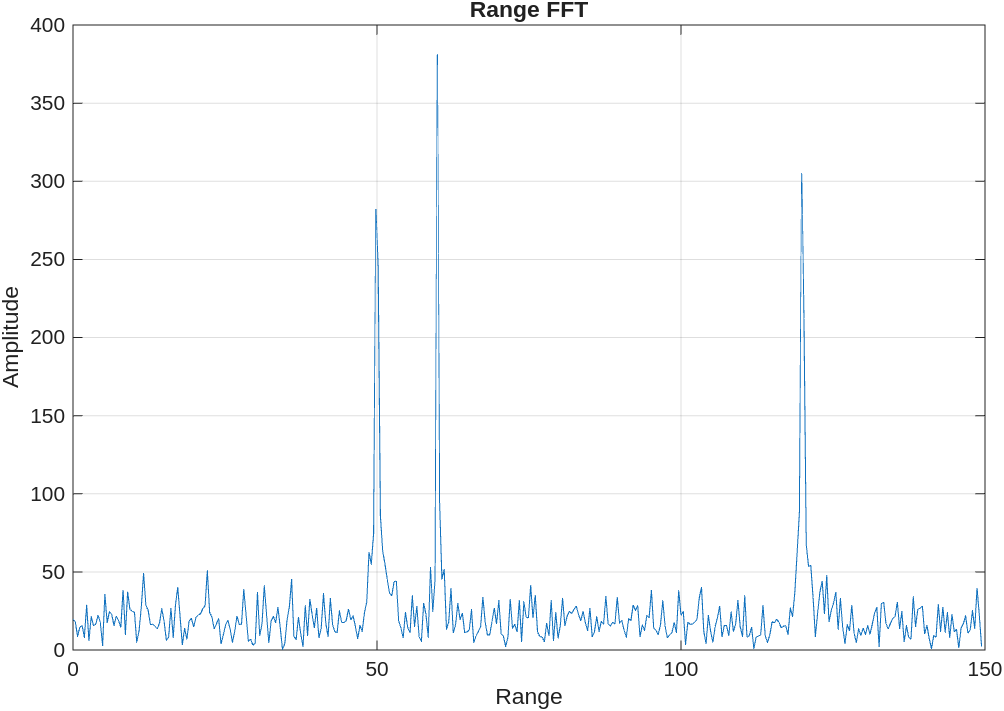
\includegraphics[width=0.6\textwidth]{figures/range-fft.png}
    \caption{Range FFT for objects at d = $\qty{50}{\meter}, \qty{60}{\meter}, \qty{120}{\meter}$}
\end{figure}

\newpage

There are limitations on the resolution and maximum distance of range detection
that are determined by the system parameters.
\begin{gather*}
    d_{res} = \frac{c}{2B} \qquad
    d_{max} = \frac{F_s c T_C}{2B}
\end{gather*}\vspace{-1.5em}
\begin{table}[H]
    \centering
    \begin{tabular}{ll}
        \toprule
        \midrule
        $B$ & Chirp bandwidth \\
        $T_C$ & Chirp period \\
        $F_s$ & Sampling frequency \\
        $f_c$ & Carrier frequency \\
        $c$ & Speed of light \\
        \bottomrule
    \end{tabular}
    \caption{Fundamental FMCW parameters and constants}
\end{table}

\section{Range-Doppler FFT}
The goal of this module is to simulate how an FMCW would determine object
velocities. Firstly, we must simulate the effect of object velocities on the
objects' range from chirp to chirp. For each chirp I defined the change in
range as
\begin{equation*}
    d_{step} = v * T_C \quad \implies \quad
    d_n = d_{n-1} + d_{step}
\end{equation*}
Velocity estimation is calculated by monitoring changes in IF phase from chirp
to chrip. Therefore, it is necessary to update the representation of the IF
signal to one that reflects its true phase.
\begin{equation*}
    IF = e^{j(2\pi f_{IF} t + \varphi)} \qquad , \qquad
    \varphi = 2\pi \frac{2d}{c} f_c
\end{equation*}
The standard way to calculate the velocities based on the phases is through the
range-Doppler matrix
\begin{gather*}
    X = \begin{bmatrix}
        FFT\left(IF_1\right) \\
        FFT\left(IF_2\right) \\
        \dots \\
        FFT\left(IF_{N_c}\right) \\
    \end{bmatrix} \quad \implies \quad
    X \in \mathbb{C}^{N_c \times N} \\\\
    Y = \begin{bmatrix}
        FFT\left(X_0\right) &
        FFT\left(X_1\right) & \dots
        FFT\left(X_N\right) \\
    \end{bmatrix} \quad \implies \quad
    Y \in \mathbb{C}^{N_c \times N}
\end{gather*}
\begin{table}[H]
    \centering
    \begin{tabular}{ll}
        \toprule
        \midrule
        $X$ & Range profiles matrix \\
        $Y$ & Range Doppler matrix \\
        $N_c$ & Num chirps considered for $v$ estimation \\
        $N$ & Num samples for FFT \\
        \bottomrule
    \end{tabular}
\end{table}
\noindent $Y$ can be presented as an image where the axis are scaled using
\begin{equation*}
    d = \frac{fc\,T_C}{2B} \quad , \quad
    v = \frac{f_{doppler} c}{2f_c}
\end{equation*}

\begin{figure}[H]
    \centering
    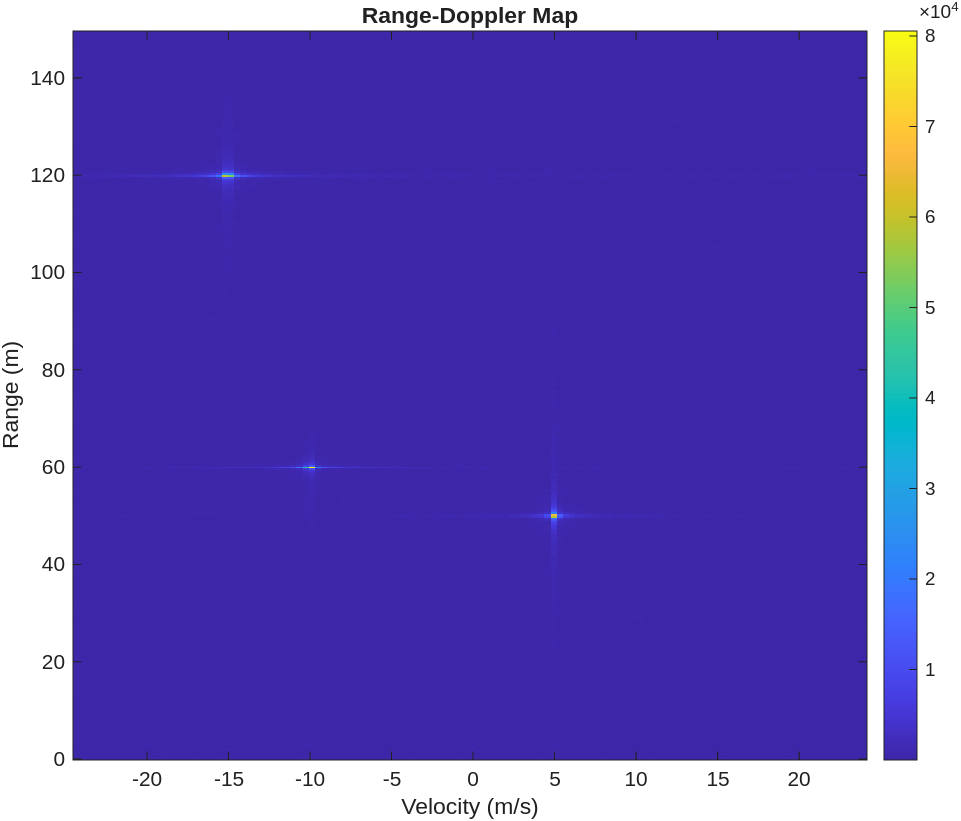
\includegraphics[width=0.6\textwidth]{figures/range-doppler.png}
    \caption{Range Doppler map for objects at $d = 50, \, 60, \, 120$ with $v = 5, -10, -15$}
    \label{fig:rd1}
\end{figure}
There are limitations on the resolution and maximum velocity of velocity
estimation that are determined by the system parameters
\begin{gather*}
    v_{res} = \frac{\lambda}{2N_c T_c} \qquad v_{max} = \frac{\lambda}{4T_c} \\
\end{gather*}

\newpage

\subsection{Realistic Target Modeling}

Due to the nature of simulating radar responses by generating representative IF
signals, the \\ Range-Doppler map is incredibly precise with narrow peaks and
low sidelobes (\ref{fig:rd1}). This section describes the steps taken in an
attempt to create a more realistic response.

\subsubsection{Target Spreading}

Generating an IF signal representative of a reflection at range $d$ doesn't match
what happens physically. In practice, an object at $d$ has some non-zero size
and sends back many reflections at slightly different times and phases. To
simulate this ranges can be "spread" by generating $N$ reflections per object
range.
\begin{gather*}
    \text{For } \mathbf{r_0}, \mathbf{v_0} \in \mathbb{R}^{n \times 1} \\\\
    \mathbf{r} = \begin{bmatrix}
        r_0 \\
        r_0 + X_1\Delta r \\
        \dots \\
        r_0 + X_N\Delta r \\
        r_1 \\
        r_1 + X_{N + 1}\Delta r \\
        \dots \\
        r_1 + X_{2N}\Delta r \\
        \dots \\
        r_n \\
        r_n + X_{(n - 1)N + 1}\Delta r \\
        \dots \\
        r_n + X_{nN}\Delta r \\
    \end{bmatrix} \qquad
    \mathbf{v} = \begin{bmatrix}
        v_0 \\
        v_0 + Y_1\Delta v \\
        \dots \\
        v_0 + Y_N\Delta v \\
        v_1 \\
        v_1 + Y_{N + 1}\Delta v \\
        \dots \\
        v_1 + Y_{2N}\Delta v \\
        \dots \\
        v_n \\
        v_n + Y_{(n - 1)N + 1}\Delta v \\
        \dots \\
        v_n + Y_{nN}\Delta v \\
    \end{bmatrix} \\\\
    X_i \sim \mathcal{U}(-1, 1) \qquad
    Y_i \sim \mathcal{U}(-1, 1)
\end{gather*}

\begin{figure}[H]
    \centering
    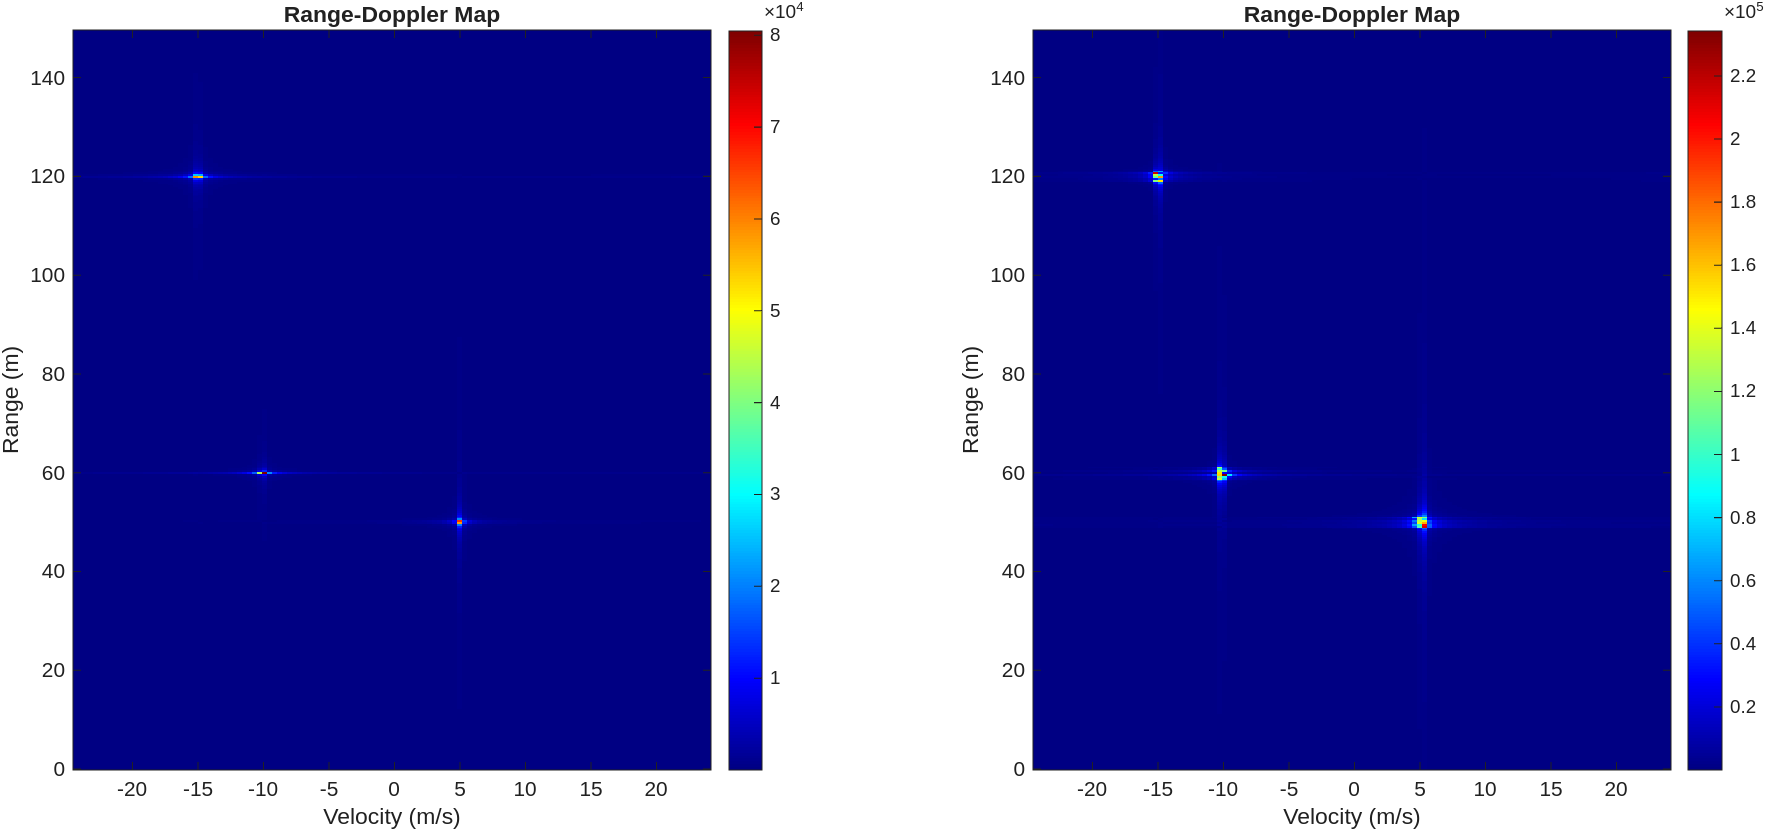
\includegraphics[width=0.8\textwidth]{figures/spreading.png}
    \caption{Nonspreading (left) vs Spreading (right)}
\end{figure}

\subsubsection{Swerling 2 RCS Fluctuation}

Another oversight of the approach so far is that it is assumed that the return
signals from the Radar Cross Section (RCS) is non-fluctuating (i.e. for an
object a given range and velocity an identical IF signal will be generated
every time).

Swerling models II and IV match the behavior of pulse to pulse (or in our case
chirp to chirp) fluctuations. Slow fluctuations or frame to frame fluctuations
would not change the behavior of our simulation because it is currently single
frame. Between models II and IV, model II is chosen because similar intensity
reflectors is standard for most targets.

\begin{table}[H]
    \centering
    \renewcommand{\arraystretch}{1.5}
    \begin{tabular}{ccccc}
        \toprule
        Model & Decorrelation & pdf of $A$ & pdf of RCS & Geometry \\
        \midrule
        I & scan-to-scan & \multirow{2}{*}{Rayleigh} & \multirow{2}{*}{Exponential}
        & \multirow{2}{2in}{\centering Several independent reflectors of similar intensity} \\
        II & pulse-to-pulse \\
        III & scan-to-scan & \multirow{2}{*}{$4^\text{th}$ order Chi} & \multirow{2}{*}{$4^\text{th}$ order Chi-square}
        & \multirow{2}{2in}{\centering Several independent reflectors and one predominates} \\
        IV & pulse-to-pulse \\
        \bottomrule
    \end{tabular}
    \caption{Characteristics of Swerling models}
\end{table}
The Rayleigh probability density function (pdf) is as follows
\begin{equation*}
    p(A) = \frac{2A}{\bar{\sigma}}\exp\left(-\frac{A^2}{\bar{\sigma}}\right)
\end{equation*}

\begin{figure}[H]
    \centering
    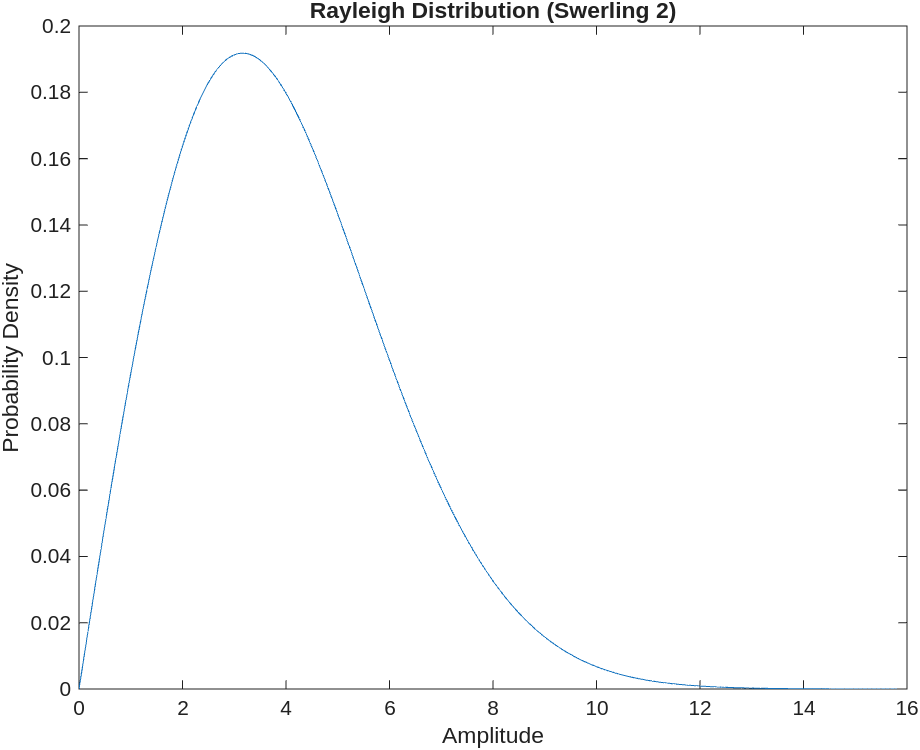
\includegraphics[width=0.6\textwidth]{figures/rayleigh.png}
    \caption{Rayleigh distribution for $\text{RCS} = 20$}
\end{figure}

\newpage

Swerling II RCS fluctuation is implemented by scaling each simulated chirp's IF
response by a different value selected from a normalized Rayleigh distribution;
resulting in a realistic smearing in velocity on the Range-Doppler map.

\begin{figure}[H]
    \centering
    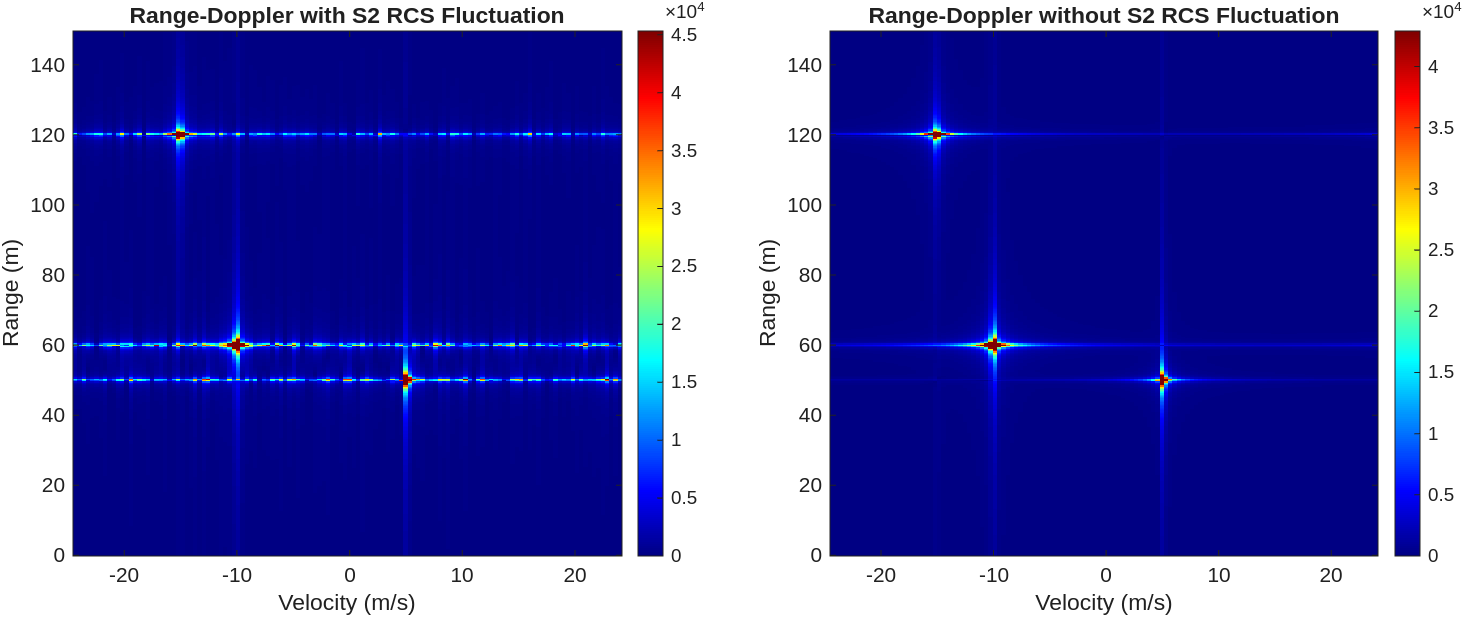
\includegraphics[width=0.9\textwidth]{figures/swerling.png}
    \caption{Range-Doppler maps with and without Swerling 2 RCS fluctuation (color scale compressed to reveal amplitude variation)}
\end{figure}


\end{document}
